\section{Toggling LEDs bottom-up}

The purpose of the first assignment is to become familiar with low level programming.
This is done by toggling LEDs using different levels of abstraction.
The sequence of this \enquote{LED show} can be seen in Table \ref{tab:led_scheme}.
Between every sequence should be a delay of approximately 1 second.

\begin{table}[H]
    \centering
    \begin{tabular}{|c|c|c|}
        \hline
        \textcolor{darkpink}{\textit{Green}} & \textcolor{darkpink}{\textit{Yellow}} & \textcolor{darkpink}{\textit{Red}}\\
        \hline
        0 & 0 & 0 \\
        \hline
        0 & 0 & 1 \\
        \hline
        0 & 1 & 0 \\
        \hline
        0 & 1 & 1 \\
        \hline
        1 & 0 & 0 \\
        \hline
        1 & 0 & 1 \\
        \hline
        1 & 1 & 0 \\
        \hline
        1 & 1 & 1 \\
        \hline
    \end{tabular}
        
    \label{tab:led_scheme}
    \caption{Order of visualisation of different LEDs}
\end{table}

As said earlier, these \enquote{LED show} should be programmed on three different levels of abstraction.
The first one is no abstraction at all using a programming technique called Direct Register Manipulation (DRM) \cite{IntroEmbeddedSystems}.
The second implementation should make use Driverlib.
The third implementation should make use of the Texas Instruments (TI) Driver.

\newpage
\subsection{Direct Register Manipulation}
\label{subsec:led_drm}

Listing \ref{lst:led_drm} shows the source code to toggle LEDs according to Table \ref{tab:led_scheme}.
The reader may wonder why the implementation of \texttt{delay\_1sec()} is missing. 
This is because it is a common function used in lots of code snippets throughout this document.
For the implementation details see Appendix \ref{subsec:appendix_delay}.
Now follows an explanation about interesting lines of code.
Line \ref{line:drm_arcm} enables the GPIOA peripheral during run mode (see Figure \ref{fig:gpio0clken}).
This program does not enter sleep mode or deep sleep mode. Setting bit 8 and bit 16 (Figure \ref{fig:gpio0clken}) does not make sense.

\begin{figure}[H]
\centering

\begin{bytefield}[endianness=big, bitwidth=3.0em]{30}
\bitheader[lsb=2]{16-31} \\
    \bitbox{15}{\tiny Reserved} &
    \colorbitbox{celadon}{1}{\tiny DSLPCLKEN} \\ [3ex]
\bitheader[lsb=-14]{0-15} \\
    \bitbox{7}{\tiny Not Used}
    \colorbitbox{celadon}{1}{\tiny SLPCLKEN}
    \bitbox{7}{\tiny Not Used}
    \colorbitbox{celadon}{1}{\tiny RUNCLKEN}
\end{bytefield}

\caption{\texttt{GPIO0CLKEN} register for the CC3220s}
\label{fig:gpio0clken}

\end{figure}

The behavior of the pins being used must be configured.
The assignment only requires the use of GPIO9, GPIO10 and GPIO11 because the built-in LEDs are routed to these pins.
Configuration for these pins are done in Line \ref{line:drm_conf9} up to and including Line \ref{line:drm_conf11}.
The value $0x60_{16}$ is written to the \texttt{GPIO\_PAD\_CONFIG\_x} register where x is 9, 10 and 11.
It affects the second nibble of the register.
Since only bit 1 and bit 2 of the nibble are affected it does not set the bit in the \texttt{open drain} field (Figure \ref{fig:padconf}).
Writing $001_{2}$ to the \texttt{DRIVE STRENGTH} field means that the related GPIO pin will drive 6 mA.

\begin{figure}[H]
\centering

\begin{bytefield}[endianness=big, bitwidth=3.0em]{30}
\bitheader[lsb=2]{16-31} \\
    \bitbox{16}{\tiny Reserved} \\ [3ex]
\bitheader[lsb=-14]{0-15} \\
    \bitbox{4}{\tiny Reserved}
    \colorbitbox{celadon}{1}{\tiny over-riding buffer}
    \colorbitbox{celadon}{1}{\tiny override value}
    \colorbitbox{celadon}{1}{\tiny pulldown}
    \colorbitbox{celadon}{1}{\tiny pullup}
    \colorbitbox{celadon}{3}{\tiny DRIVE STRENGTH}
    \colorbitbox{celadon}{1}{\tiny open drain}
    \colorbitbox{celadon}{4}{\tiny CONFMODE}
\end{bytefield}

\caption{\texttt{GPIO\_PAD\_CONFIG\_x} register for the CC3220s}
\label{fig:padconf}

\end{figure}

A GPIO pin is either input or output. Writing a 1 to the \texttt{GPIO\_DIR} register (Figure \ref{fig:dirconf}) configures a GPIO pin as output pin.
Writing a 0 to the \texttt{GPIO\_DIR} register configures a GPIO pin as input pin.
Because this program only needs GPIO9, GPIO10 and GPIO11 the program needs to write a 1 to bit 1, bit 2 and bit 3 respectively.
$00001110_{2}$ is $0x0E_{16}$ in hexadecimal representation.
That is why the program writes $0x0E_{16}$ to the \texttt{GPIO\_DIR} register at Line \ref{line:drm_dir}.

\begin{figure}[H]
\centering

\begin{bytefield}[endianness=big, bitwidth=3.0em]{30}
\bitheader[lsb=2]{16-31} \\
    \bitbox{16}{\tiny Reserved} \\ [3ex]
\bitheader[lsb=-14]{0-15} \\
    \bitbox{8}{\tiny Reserved}

    \colorbitbox{celadon}{1}{\tiny DIR}
    \colorbitbox{celadon}{1}{\tiny DIR}
    \colorbitbox{celadon}{1}{\tiny DIR}
    \colorbitbox{celadon}{1}{\tiny DIR}
    \colorbitbox{celadon}{1}{\tiny DIR}
    \colorbitbox{celadon}{1}{\tiny DIR}
    \colorbitbox{celadon}{1}{\tiny DIR}
    \colorbitbox{celadon}{1}{\tiny DIR}

\end{bytefield}

\caption{\texttt{GPIO\_DIR} register for the CC3220s}
\label{fig:dirconf}

\end{figure}

Setting the output pin to logic high or logic low requires a little extra explanation.
There is a mask which should be added to the base address plus the address of the \texttt{GPIO\_DATA} register.
This prevents software from a read-modify-write operation. A change in logic level of an GPIO output pin is done in a single cycle.
The bits one would like to change should be shifted 2 positions to the right and added to base address + the \texttt{GPIO\_DATA} offset.
Line \ref{line:drm_init_data} turns the three LEDs off by writing $00000000_{2}$ or $0x00_{16}$ to the \texttt{GPIO\_DATA} register.
However, because of the mask added to the address only bit 1, bit 2 and bit 3 are affected.

\begin{figure}[H]
\centering

\begin{bytefield}[endianness=big, bitwidth=3.0em]{30}
\bitheader[lsb=2]{16-31} \\
    \bitbox{16}{\tiny Reserved} \\ [3ex]
\bitheader[lsb=-14]{0-15} \\
    \bitbox{8}{\tiny Reserved}

    \colorbitbox{celadon}{1}{\tiny DATA}
    \colorbitbox{celadon}{1}{\tiny DATA}
    \colorbitbox{celadon}{1}{\tiny DATA}
    \colorbitbox{celadon}{1}{\tiny DATA}
    \colorbitbox{celadon}{1}{\tiny DATA}
    \colorbitbox{celadon}{1}{\tiny DATA}
    \colorbitbox{celadon}{1}{\tiny DATA}
    \colorbitbox{celadon}{1}{\tiny DATA}

\end{bytefield}

\caption{\texttt{GPIO\_DATA} register for the CC3220s}
\label{fig:dataconf}

\end{figure}

The following things happen in an infinite loop.
Line \ref{line:drm_toggle} in Listing \ref{lst:led_drm} write a variable \texttt{index} to \texttt{GPIO\_DATA} register.
This value is shifted 1 position to the left because the first LED is positioned at GPIO9 and not at GPIO8.
Line \ref{line:drm_modulo} increments \texttt{index}. Variable \texttt{index} can hold $0 \leq index < 16$ (although $0 \leq index < 8$ would be sufficient).
The second operand of the modulo operator does not really matter as long as it is a multiple of $2^3$.
Line \ref{line:drm_sleep} makes a call to \texttt{delay\_1sec()}. The function returns after 1 second since it is a busy-wait like implementation where the CPU just burns CPU cycles.

\begin{lstlisting}[style=CStyle, caption={Toggling LEDs according to Table \ref{tab:led_scheme} using DRM programming technique}, captionpos=b, label={lst:led_drm}, escapechar=@]
#include <stdint.h>
#include <stddef.h>
#include "register_def.h"
 
#include "inc\hw_memmap.h"
#include "inc\hw_gpio.h"
#include "inc\hw_apps_rcm.h"
#include "inc\hw_ocp_shared.h"
 
/* Function delay_1sec() used to be here */

int main(void)
{
 
    HWREG(ARCM_BASE + APPS_RCM_O_GPIO_A_CLK_GATING) = 0x01; @\label{line:drm_arcm}@
 
    HWREG(OCP_SHARED_BASE + OCP_SHARED_O_GPIO_PAD_CONFIG_9) = 0x60; @\label{line:drm_conf9}@
    HWREG(OCP_SHARED_BASE + OCP_SHARED_O_GPIO_PAD_CONFIG_10) = 0x60; @\label{line:drm_conf10}@
    HWREG(OCP_SHARED_BASE + OCP_SHARED_O_GPIO_PAD_CONFIG_11) = 0x60; @\label{line:drm_conf11}@
 
    HWREG(GPIOA1_BASE + GPIO_O_GPIO_DIR) = 0x0E;    @\label{line:drm_dir}@
    HWREG(GPIOA1_BASE + GPIO_O_GPIO_DATA + (0x0E << 2)) = 0x00; @\label{line:drm_init_data}@
 
    int index = 0;
 
    while(1)
    {
        HWREG(GPIOA1_BASE + GPIO_O_GPIO_DATA + (0x0E << 2)) = (index << 1); @\label{line:drm_toggle}@
        index = (index + 1) % 16;       @\label{line:drm_modulo}@
        delay_1sec();                   @\label{line:drm_sleep}@
    }
 
    return 0;
}
\end{lstlisting}


\newpage
\subsection{Driverlib}

Driverlib is a library which provides access to peripherals.
The advantage of this is that the programmer does not need to know base addresses and offsets in order to access special function registers.
Line \ref{line:driverlib_clk} in Listing \ref{lst:led_driverlib} enables the \texttt{GPIOA1} peripheral by enabling a clock signal to the peripheral.
Line \ref{line:driverlib_pad1} up to and including Line \ref{line:driverlib_pad3} configures the GPIO9, GPIO10 and GPIO11 pin characteristics. The pins can use now a maximum of 2 mA per pin.
Note that the function accepts a macro which contains the physical pin number instead of the logical pin number.
Line \ref{line:driverlib_dir1} up to and including Line \ref{line:driverlib_dir3} configures GPIO9, GPIO10 and GPIO11 to an output pin.
Line \ref{line:driverlib_data1} up to and including Line \ref{line:driverlib_data3} turns the three LEDs off by default.

Line \ref{line:driverlib_toggle} writes the value \texttt{switcher} to the \texttt{GPIO\_DATA} register but only \texttt{GPIO\_PIN\_1}, \texttt{GPIO\_PIN\_2} and \texttt{GPIO\_PIN\_3} (which are GPIO9, GPIO10 and GPIO11) are sensitive for this value change. 
Line \ref{line:driverlib_sleep} makes a function call to \texttt{delay\_1sec()} which will return to the caller after 1 second.

\begin{lstlisting}[style=CStyle, caption={Toggling LEDs according to Table \ref{tab:led_scheme} using Driverlib library}, captionpos=b, label={lst:led_driverlib}, escapechar=@]
#include <stdint.h>
#include <stddef.h>
#include "register_def.h"
 
#include "gpio.h"
#include "pin.h"
#include "prcm.h"
 
/* GPIO 9 is PIN_64 is (red) */
/* GPIO 10 is PIN_2 is (green) */
/* GPIO 11 is PIN_1 is (yellow) */
 
/* Function delay_1sec() used to be here */
 
int main(void)
{
    PRCMPeripheralClkEnable(PRCM_GPIOA1 ,PRCM_RUN_MODE_CLK);        @\label{line:driverlib_clk}@
 
    PinTypeGPIO(PIN_64, PIN_STRENGTH_2MA, false);   /* Red LED is push-pull */  @\label{line:driverlib_pad1}@
    PinTypeGPIO(PIN_01, PIN_STRENGTH_2MA, false);   /* Yellow LED is push-pull */ @\label{line:driverlib_pad2}@
    PinTypeGPIO(PIN_02, PIN_STRENGTH_2MA, false);   /* Green LED is push-pull */  @\label{line:driverlib_pad3}@
 
    GPIODirModeSet(GPIOA1_BASE, GPIO_PIN_2, GPIO_DIR_MODE_OUT); @\label{line:driverlib_dir1}@
    GPIODirModeSet(GPIOA1_BASE, GPIO_PIN_3, GPIO_DIR_MODE_OUT); @\label{line:driverlib_dir2}@
    GPIODirModeSet(GPIOA1_BASE, GPIO_PIN_1, GPIO_DIR_MODE_OUT); @\label{line:driverlib_dir3}@
 
    GPIOPinWrite(GPIOA1_BASE, GPIO_PIN_2, ~GPIO_PIN_2);  /* Turn yellow LED off */ @\label{line:driverlib_data1}@
    GPIOPinWrite(GPIOA1_BASE, GPIO_PIN_3, ~GPIO_PIN_3);  /* Turn green LED off */   @\label{line:driverlib_data2}@
    GPIOPinWrite(GPIOA1_BASE, GPIO_PIN_1, ~GPIO_PIN_1);  /* Turn red LED off */    @\label{line:driverlib_data3}@
 
    int switcher = 0;
 
    while(1)
    {
        GPIOPinWrite(GPIOA1_BASE, GPIO_PIN_1 | GPIO_PIN_2 | GPIO_PIN_3, switcher);  @\label{line:driverlib_toggle}@
        delay_1sec();                                                               @\label{line:driverlib_sleep}@
 
        switcher = (switcher + 1) % 16;                                             @\label{line:driverlib_inc}@
    }
}
\end{lstlisting}

\newpage
\subsection{TI Driver}

TI Driver is a library which provides access to peripherals.
The advantage of this is that the programmer does not need to know base addresses and offsets in order to access special function registers.
Line \ref{line:ti_init} in Listing \ref{lst:led_ti} enables the GPIOA peripheral.
Line \ref{line:ti_out1} up to and including Line \ref{line:ti_out3} configures the GPIO pins wired to the LEDs as output pins.
Line \ref{line:ti_off1} up to and including Line \ref{line:to_off3} turns the LEDs off by default.

Line \ref{line:ti_set1} up to and including Line \ref{line:ti_set3} set GPIO9, GPIO10 and GPIO11 respectively.
The function \texttt{GPIO\_write()} its second parameter accepts either a 1 or 0 according to the documentation generated by Doxygen. 
That is why there are masks and bit shifts.
Line \ref{line:ti_sleep} calls the \texttt{delay\_1sec()} function which waits 1 second before returning to the caller.
Variable \texttt{switcher} is incremented (Line \ref{line:ti_inc}) modulo 8 to make sure no overflow will happen. 

\begin{lstlisting}[style=CStyle, caption={Toggling LEDs according to Table \ref{tab:led_scheme} using TI Driver}, captionpos=b, label={lst:led_ti}, escapechar=@]
void *mainThread(void *arg0)
{
    /* Call driver init functions */
    GPIO_init();        @\label{line:ti_init}@
 
    /* Configure the LED */
    GPIO_setConfig(Board_GPIO_LED0, GPIO_CFG_OUT_STD | GPIO_CFG_OUT_LOW); @\label{line:ti_out1}@
    GPIO_setConfig(Board_GPIO_LED1, GPIO_CFG_OUT_STD | GPIO_CFG_OUT_LOW); @\label{line:ti_out2}@  
    GPIO_setConfig(Board_GPIO_LED2, GPIO_CFG_OUT_STD | GPIO_CFG_OUT_LOW); @\label{line:ti_out3}@
 
    /* Turn off user LED */
    GPIO_write(Board_GPIO_LED0, Board_GPIO_LED_OFF);    /* Turn red LED off */ @\label{line:ti_off1}@
    GPIO_write(Board_GPIO_LED1, Board_GPIO_LED_OFF);    /* Turn yellow LED off */ @\label{line:ti_off2}@
    GPIO_write(Board_GPIO_LED2, Board_GPIO_LED_OFF);    /* Turn green LED off */ @\label{line:to_off3}@
 
    unsigned int switcher = 0;
 
    while(1)
    {
        GPIO_write(Board_GPIO_LED0, switcher & 1);      @\label{line:ti_set1}@
        GPIO_write(Board_GPIO_LED1, (switcher & 2) >> 1);   @\label{line:ti_set2}@
        GPIO_write(Board_GPIO_LED2, (switcher & 4) >> 2);   @\label{line:ti_set3}@
        delay_1sec();                                   @\label{line:ti_sleep}@
 
        switcher = (switcher + 1) % 8;  @\label{line:ti_inc}@
    }
 
 
    return (NULL);
}
\end{lstlisting}


\newpage
\subsection{Verification of the behaviour using a logic analyzer}

The behavior of the programs must be verified to be able to determine with certainty whether the requirements of the assignment has been met.
This verification is done using a logic analyzer.
The logic analyzer has been used for all three programs, but the results are almost the same.
That is why there are only three figures instead of nine.
Figure \ref{fig:led_togglee1} up to and including Figure \ref{fig:led_togglee3} are the same snapshot but the mouse hovers different channels to pop up extra information.
Channel 0 is the red LED, channel 1 is the yellow LED and channel 2 is the green LED.

\begin{figure}[H]
\centering
    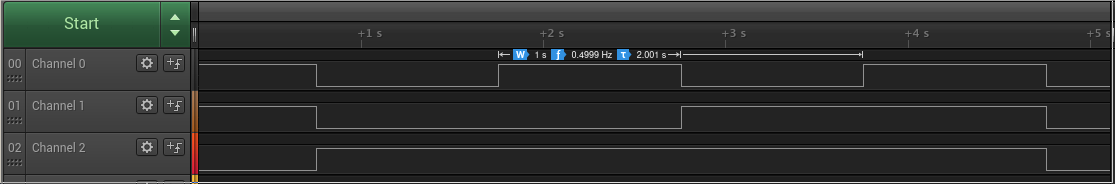
\includegraphics[scale=0.4]{img/led_toggle1.png}
\caption{The red LED is toggled every second}
\label{fig:led_togglee1}

\end{figure}

\begin{figure}[H]
\centering
    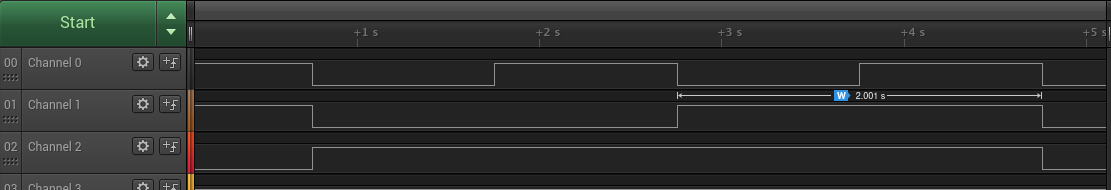
\includegraphics[scale=0.4]{img/led_toggle2.png}
\caption{The yellow LED is toggled every two seconds (twice as much as the red LED)}
\label{fig:led_togglee2}

\end{figure}

\begin{figure}[H]
\centering
    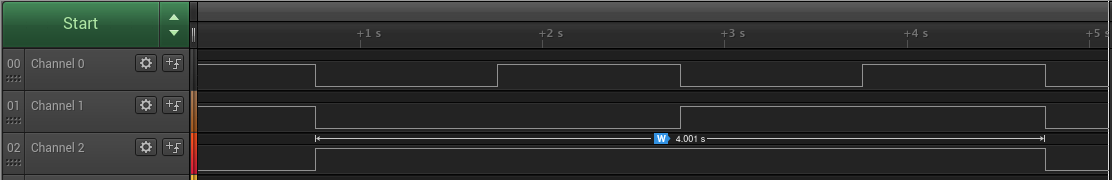
\includegraphics[scale=0.4]{img/led_toggle3.png}
\caption{The green LED is toggled every four seconds (twice as much as the yellow LED)}
\label{fig:led_togglee3}

\end{figure}
